\documentclass[a4paper]{article}
\usepackage{listings}
\usepackage{graphicx}
%\usepackage[scale=.7]{geometry}
\usepackage{amsmath}
\usepackage{float}
\usepackage{acronym}
\usepackage{cite}
\usepackage{url}
\usepackage[usenames, pdftex]{color}

\acrodef{WSM}[WSM]{Weighted Scan Matching}
\acrodef{ICP}[ICP]{Iterated Closest Point}
\acrodef{RANSAC}[RANSAC]{Random Sample Consensus}
\acrodef{PFH}[PFH]{Point Feature Histograms}
\acrodef{FPFH}[FPFH]{Fast Point Feature Histograms}
\acrodef{SLAM}[SLAM]{Simultaneous Localization and Mapping}
\acrodef{PCL}[PCL]{Point Cloud Library}
\acrodef{SAC-IA}[SAC-IA]{SAmple Consensus Initial Alignment}

\title{Registration using RGB-D camera\\
{\large Project A.I. / Individual project}}

\author{Carsten van Weelden \\ 0518824 \\ \texttt{cvanweelden@gmail.com} \and Thomas van den Berg \\ 5789346 \\ \texttt{Thomas.G.vandenBerg@gmail.nl} \and
 \small{Supervisor:} \\ Arnoud Visser \\ University of Amsterdam\\
  The Netherlands}

\date{\today}




\begin{document}
\maketitle



\section{Introduction}

In this project we familiarized ourselves with several methods for 3D registration. The availability of cheap RGB+D sensors such as the Kinect could lead to new applications. A Kinect mounted on a moving robot could replace both it's RGB camera and it's range finder. A new application could be affordable 3D reconstructions of the insides of buildings. But in order to make sense of the Kinect's output, we need to perform a registration step; we need to \emph{register} the output of the RGB+D camera, i.e, we need to find the transformation that the camera made in between the captured frames. The robot's odometry can sometimes be used to get an initial estimate of the transformation, but in a scenario where the RGB+D camera is hand-held not even this is possible. For this reason we focused on the registration step only. 

The combined RGB and depth data forms a ``point cloud'': a set of 3D coordinate points indicating where the sensor measured a solid object. Assuming that there is enough overlap between each pair of consecutive point clouds, we find a good registration by finding an optimal way to fit the two clouds. We've experimented with different registration methods, and we'll report on their performance and whether it degrades under certain circumstances.

\section{Background}

\subsection{Registration}

\subsubsection{ICP Based Registration}

A basic method used in almost every approach to 3D registration is \ac{ICP}\cite{besl1992method}, it is an expectation maximization method that iteratively minimizes the distance between each point and it's closest neighbor. Though \ac{ICP} is currently used mostly as a refinement step for more advanced algorithms, there are still some papers describing experiments where using \ac{ICP} as the main registration procedure has been successful [[WHICH]]. 

In \cite{segal2009generalized}, an extension to \ac{ICP} was introduced that takes into account the local characteristics of the matched points. This Generalized-ICP gives a higher weight to point correspondence errors if they are in a direction perpendicular to the estimated plane. It is mentioned in both \cite{rusinkiewicz2001efficient} and \cite{segal2009generalized} that using this extension prevents the application of a closed-form solution to the minimization step.

\ac{WSM} removes a simplyfying assumption from \ac{ICP}, namely that ``the range scans of different poses sample the environment's boundary at \emph{exactly} the same points''~\cite{pfister2002weighted}. In range scans, it often occurs that the points are much further apart in some areas of the model, because of the angle of the local surface or the distance from the sensor. The point-to-point error in these areas could easily be much greater, this is what the authors take into account by introducing an error which they name the \emph{correspondence error}. They model the variance of this error based on the distances to the closest model points, \cite{slamet2008boosting} give a clear illustration in their Figure 1. 

In a sense, Generalized-ICP and \ac{WSM} are similar in that they make an explicit model of the error that the minimization step aims to minimize, based on the local characteristics. This has some clear advantages in terms of accuracy, but the extra computational costs are significant.

\subsubsection{Feature Based Registration}

An alternative to \ac{ICP} based registration is feature-based registration in which the transformation between frames is estimated from correspondences between feature points in 3D space, usually combined with \ac{RANSAC}. In stead of matching each point in the cloud to it's closest neighbour, characteristic points are extracted, and a feature \emph{descriptor} is calculated for each. Based on these descriptors, the feature points are matched to their counterparts in the other frame to get a number of \emph{correspondences}. Not all these correspondences may be correct though, so \ac{RANSAC} is often used to filter the outliers. 

\cite{rusu2009fast} describes such an approach. In it, \ac{PFH} are used as feature descriptors. For each point, these features are based on the properties of points in its neighborhood. To elaborate, every pair of points within the neighborhood (Figure~\ref{fig:fpfh}) generates a number of features based on their angle with respect to the local normal. Because the number of neighbors can vary, a histogram is created. Initially, every single point is used to generate a descriptor. Then, to speed up the matching and make it more robust, only \emph{unique} feature points are selected, i.e. points whose descriptors are different from the mean descriptor. \ac{RANSAC} is then used to find the best feature point correspondences.  

\begin{figure}[htbp]
    \centering
        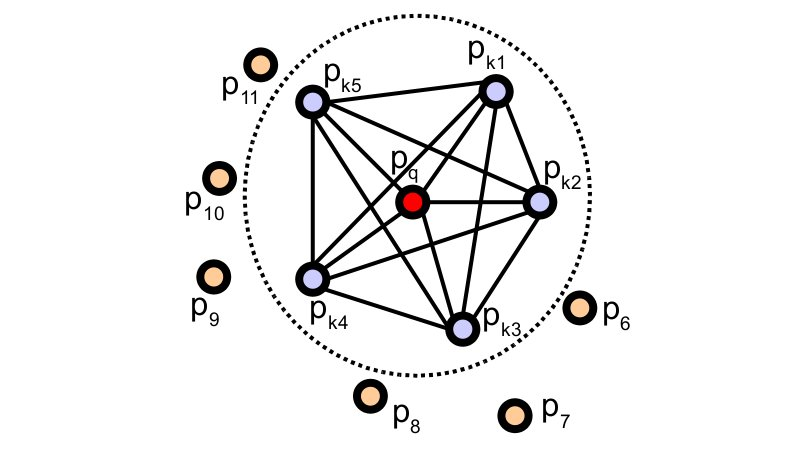
\includegraphics[height=4cm]{ims/fpfh.jpg}
    \caption{The PFH dependency diagram (image from \cite{rusu2009fast}). It indicates that every pair of points in the neighborhood generates features.}
    \label{fig:fpfh}
\end{figure}

\subsection{Applications}

\subsubsection{Global registration}

Global registration is the problem of reconstructing a global model from a sequence of frames. Each frame has to be registered to a global coordinate system, generally defined by the axes of the first frame of the sequence. One challenge in applying registration algorithms to this problem is that errors in pairwise registration accumulate over time. Other challenges associated with global registration are integrating the registered noisy measurements into a smooth global model and dealing with dynamic scenes in which objects move between frames.

In the KinectFusion project presented in \cite{izadi2011kinectfusion,newcombe2011kinectfusion} \ac{ICP} is used to register depth frames captured using a Kinect camera to build a global model. For the model they use the volumetric representation described in \cite{curless1996volumetric}. 
%Explain how this deals with registration noise and error build up.

\subsubsection{\ac{SLAM}}

As mentioned before, the registration step that we focus on in this report provides us with all the information needed to perform \ac{SLAM}. By finding the relative transformation between frames we can compute the new position of the camera (localization), and by merging the 3D images we create a map of the environment. This is also know as \emph{visual odometry} and a more complete overview can be found in \cite{scaramuzzavisual,fraundorfervisual}. Like global registration, it suffers from the accumulated error from pairwise registration and is generally combined with global optimization techniques such as loop closing to generate an accurate camera trajectory. However, though the registration step is essential, it is far from sufficient for good localization. The most notable problem is the \emph{error buildup}; cumulative errors in the registration steps cause an ever greater error in the final position estimation. This can lead to a defective \emph{loop closing}: when the sensor comes to a place it has been before, the built-up error will almost surely cause this to be registered as a different position from the original one. If this d\'ej\`a-vu can be detected at all, it is still necessary to re-register all earlier frames so that the loop is ``straightened out''.

%In \cite{pfingsthorn2008scalable} \ac{WSM} is combined with loop closing and a manifold data structure?

In \cite{slamet2008boosting} \ac{ICP} and \ac{WSM} are applied to solve the \ac{SLAM} problem in 2D, but instead of registering each frame to the previous frame they store all registered frames in a quad tree and register the frames against multiple previously registered frames. They show that this leads to better results than incremental pair-wise registration of frames.

In \cite{nuchter20076d} \ac{ICP} is used on point cloud data to solve the \ac{SLAM} problem in 3D. They use a cached version of the kd-tree data structure to make this feasible in real-time. They state that in combination with loop closing and model refinement this leads to accurate results.

\section{Experiments}

We ran a number of experiments to find out about the behavior of different registration methods and their performance in different settings. One of the most influential properties of the input data is the magnitude of the transformation between frames. To clarify; a slow-driving robot will record frames that are are mostly similar, making it easier to find corresponding points or features in both frames, whereas a shaky handheld RGB-D camera might output frames with a much larger discrepancy. Typically, a set of frames with small transformations between them is an easier input to a registration algorithm. However, when building a global model or using the registration to perform SLAM, each step contributes an amount of error to the final results, therefore it is better to use as few frames as possible as long as the registration still works reasonably well. [[Is er een artikel waar ze frames overslaan onder bepaalde condities?: dat even citeren.]]

Our first experiment examines whether the total buildup of error is larger when using more frames, we did this by [[...]] We've also run the registration on the dataset to create a global model, to show that the buildup of error can be quite catastrophic for this purpose.

The rest of our experiments focus on the advantages of using feature-based registration methods when the magnitude of the relative transform between frames gets larger. All of these experiments consist of registering each frame $i$ to the $i-n^{\mathrm{th}}$ frame, with $n = 1,2,3,...$. By skipping frames in this manner, we artificially create a larger transformation for the registration step to solve. We expect to see that the feature-based methods are better at dealing with this larger transformation.

\subsection{Datasets}

We use two RGB-D datasets from the benchmark presented in \cite{sturm11rss-rgbd}. In addition to the RGB-D data, it contains a ground truth for the camera's position obtained using a motion capture system which we use for evaluation. Both datasets are captured as an indoor scene around a desk with several objects on it.

The specific datasets that we use are \texttt{freiburg2\_xyz} and \texttt{freiburg1\_desk}\footnote{Available at \url{http://cvpr.in.tum.de/data/datasets/rgbd-dataset}}. The \texttt{xyz} dataset was recorded with a slow and steady movement of the RGB-D sensor, so that the magnitude of the translation is constant. Rotation is kept to a minimum. The \texttt{desk} dataset is recorded with much faster movement, leading to larger differences between subsequent frames as well as motion blur and rolling shutter effects. It contains both translation and rotation between frames.

\subsection{Implementation}

For our implementation we use \ac{PCL} \cite{Rusu_ICRA2011_PCL}. We use the standard \ac{ICP} implementation provided by this library with a maximum of 25 iterations and maximum correspondence distance of 0.25m. For our feature based method we use the implementation of the \ac{SAC-IA} method from \cite{rusu2009fast} as implemented for this library\footnote{This implementation does not apply the Levenberg-Marquardt algorithm as described in the paper. In stead, we apply the \ac{ICP} algorithm as final refinement.}, limited to 1000 iterations with a maximum correspondence distance of 0.1m and minimum distance of 0.5m between the samples used for the \ac{RANSAC} method. For the \ac{FPFH} features we use a radius of 0.1m for normal estimation and 0.5m for feature computation. In all cases we remove sparse outliers by removing all points whose mean distance to its 50 nearest neighbors is more than one standard deviation from the overall mean and we subsample by taking one point for each 5cm$^3$ voxel.





\subsection{Accumulated error over time}
\label{accumulated_error}

The registration step registers a pair of frames with a certain error (which we investigate in section \ref{registration_error}. For global registration and \ac{SLAM} this error accumulates as frames are sequentially registered to previously registered frames. One way to deal with this problem is by skipping frames. Registering fewer frames means accumulating less error, but the overlap between the frames need to be large enough for successful registration. 

We investigate the effect of skipping frames by looking at the registration error after a fixed duration with varying offsets between registered frames. We calculate the mean error over 50 segments of 2 seconds starting at frame 1 to 50 for the \texttt{freiburg2\_xyz} and \texttt{freiburg1\_desk} datasets.

\subsubsection{Results}


\subsection{Registration error}
\label{registration_error}

We show how the error for registering a frame pair increases as the frames are farther apart by computing the rotation and translation error for frame pairs with varying offsets between frames. Here we use the frame offset as a proxy for the magnitude of the transformation, but we also show how the rotation and translation magnitudes vary with the frame offset.

We calculate the rotation error as the angular distance between the true rotation $q$ and the estimated rotation $\hat q$ which we calculate as $min(\theta, 2\pi - \theta)$ where $\theta$ is the angle between the two rotations represented as quaternions: $\theta = 2 * cos^{-1}(q \cdot \hat q)$. %Dit hierboven heb ik opgeschreven omdat het nergens te vinden was.
The translation error is given as the euclidean norm of the difference between the true and estimated translation. We compute the mean errors over 50 frame pairs for up to 2 seconds apart from the start of the \texttt{freiburg2\_xyz} and \texttt{freiburg1\_desk} datasets.

\subsubsection{Results}


%\section{Results}

[[Laten zien dat de error buildup ervoor zorgt dat een globaal model een zootje wordt, op onze eigen dataset]]

[[Grafiek die laat zien dat de error van A->B + B->C groter is dan van A->C, dat het dus zin heeft om frames te skippen]]

[[Grafiek die laat zien \emph{hoe groot} de transformaties zijn die ICP inschat, vergeleken bij de ground truth: misschien toont dat aan dat ICP altijd liever kleine transformaties kiest]]
[[In dezelfde grafiek: met een feature based methode]]

[[Grafiek met de gemiddelde relative error van ICP en van Feature-Based voor verschillende frameskips]]
[[Idem, voor andere dataset]]

[[Grafiek die laat zien dat ICP minder iteraties nodig heeft als er een Feature-Based stap aan vooraf gaat]]

\section{Discussion}

% Why does pure ICP work in the other articles? How do we show this?

% Analysis of featurebased methods

% Why u no use color?


\bibliography{../../literature/refs}{}
\bibliographystyle{apalike}

\end{document}
